\documentclass{article}
\usepackage{microtype,graphicx,subcaption,booktabs,hyperref,amsmath,amssymb,xcolor}
\usepackage{tikz}
\usetikzlibrary{positioning,arrows.meta,fit}
\usepackage[accepted]{icml2025}
\newcommand{\todo}[1]{\textcolor{red}{[TODO: #1]}}
\icmltitlerunning{BioFool: Fooling BioCLIP with Generated Images}

\begin{document}
\twocolumn[
\icmltitle{BioFool: Semantic Adversarial Image Generation\\against a Tree-of-Life Foundation Model}
\begin{icmlauthorlist}
\icmlauthor{\todo{Author 1}}{uni}
\icmlauthor{\todo{Author 2}}{uni}
\icmlauthor{\todo{Author 3}}{uni}
\end{icmlauthorlist}
\icmlaffiliation{uni}{\todo{University}}
\icmlcorrespondingauthor{\todo{Name}}{\todo{email}}
\icmlkeywords{diffusion models, adversarial examples, reinforcement learning, BioCLIP}
\vskip 0.3in
]
\printAffiliationsAndNotice{}

\begin{abstract}
BioCLIP is a vision--language foundation model that names organisms across the whole tree of life, and it is used
to support biodiversity monitoring. We ask how robust it is to realistic images it has never seen. We build
\emph{BioFool}, a generative application that produces faithful images of a given species that BioCLIP's public
open-set classifier ($\sim$450k species) gets wrong. Fidelity is judged by GPT-4o, a model of another family, and
by humans. We adapt Stable Diffusion in four ways: context engineering of the prompt (including an LLM attacker),
editing of real photographs, inference-time search with a new \emph{early-rejection} scheme, and post-training of a
LoRA with reinforcement learning (DDPO with group-relative advantages). We then accelerate sampling. On four datasets
(synthetic images, iNaturalist photos, invasive species and BioCLIP's own Rare Species benchmark), \todo{headline
result: e.g. DDPO raises the attack success rate from X\% to Y\% on unseen species; early rejection keeps Z\% of
best-of-N's gain at 55\% of its cost}. Code: \url{\todo{repository URL}}.

\end{abstract}

\section{Introduction}
Foundation models for biology such as BioCLIP~\citep{stevens2024bioclip} classify images of organisms zero-shot at
any rank of the taxonomy. They are integrated into citizen-science tools, camera-trap pipelines and the detection of
invasive species, where a confident wrong name has a cost. Standard benchmarks measure accuracy on curated photos;
they say little about the images such a tool meets in practice: unusual backgrounds, night flash, larvae instead of
adults, partial views, or deliberately misleading pictures.

We study this question with generative models. Our application produces \emph{semantic} adversarial examples: images
that a person (and an independent model) recognises as species $y$, but on which BioCLIP outputs another species.
Unlike pixel-level attacks~\citep{szegedy2014intriguing}, these images are plausible photographs; they are in the
spirit of unrestricted~\citep{song2018constructing} and natural~\citep{hendrycks2021natural} adversarial examples.

Our definition makes the problem well posed: an image only counts as an attack if an evaluation oracle that is
independent of the training signal confirms the species (Section~\ref{sec:method}). Without this condition, a generator
can trivially ``fool'' the classifier by drawing badly; an RL-trained generator learns exactly that (we show it).

\textbf{Contributions.}
(i) A pipeline that attacks the real, open-set BioCLIP with text-to-image and image-to-image generation, on four
datasets.
(ii) A post-training method: DDPO~\citep{black2024ddpo} with group-relative advantages~\citep{shao2024deepseekmath}
and a two-oracle reward, which generalises to species unseen in training.
(iii) An inference-time improvement, \emph{early rejection}, that prunes best-of-$N$ candidates from a cheap preview
of the predicted clean image, and a study of sampling acceleration.
(iv) An analysis of \emph{where} BioCLIP fails: per context family, per taxonomic rank, in its embedding space and in
its saliency maps. Figure~\ref{fig:pipeline} summarises the approach.

\begin{figure}[t]
\centering
\resizebox{\columnwidth}{!}{% Summary figure of the report. \usepackage{tikz} \usetikzlibrary{positioning,arrows.meta,fit}
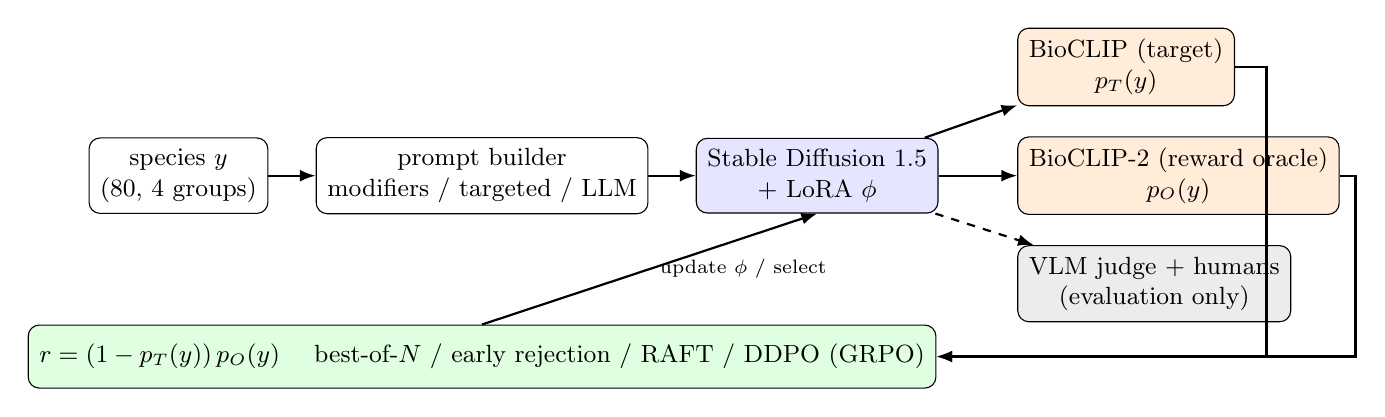
\begin{tikzpicture}[
  box/.style={draw, rounded corners, align=center, font=\small, minimum height=8mm, inner sep=4pt},
  gen/.style={box, fill=blue!10}, clf/.style={box, fill=orange!15}, opt/.style={box, fill=green!12},
  arr/.style={-{Latex[length=2mm]}, thick}]
  \node[box] (sp) {species $y$\\(80, 4 groups)};
  \node[box, right=6mm of sp] (pr) {prompt builder\\modifiers / targeted / LLM};
  \node[gen, right=6mm of pr] (sd) {Stable Diffusion 1.5\\+ LoRA $\phi$};
  \node[clf, above right=4mm and 10mm of sd] (t) {BioCLIP (target)\\$p_T(y)$};
  \node[clf, right=10mm of sd] (o) {BioCLIP-2 (reward oracle)\\$p_O(y)$};
  \node[clf, below right=4mm and 10mm of sd, fill=gray!15] (e) {VLM judge + humans\\(evaluation only)};
  \node[opt, below=14mm of pr, minimum width=60mm] (r) {$r=(1-p_T(y))\,p_O(y)$ \quad best-of-$N$ / early rejection / RAFT / DDPO (GRPO)};
  \draw[arr] (sp) -- (pr);
  \draw[arr] (pr) -- (sd);
  \draw[arr] (sd) -- (t);
  \draw[arr] (sd) -- (o);
  \draw[arr, dashed] (sd) -- (e);
  \draw[arr] (t.east) -| ++(4mm,-30mm) |- (r.east);
  \draw[arr] (o.east) -| ++(2mm,-14mm) |- (r.east);
  \draw[arr] (r.north) -- node[right, font=\scriptsize]{update $\phi$ / select} (sd.south);
\end{tikzpicture}
}
\caption{BioFool. A prompt (or a real photo) is turned into an image by Stable Diffusion with a LoRA. BioCLIP (the
target) and BioCLIP-2 (the reward oracle) score it; the reward drives search and RL. Reported fidelity comes from a
separate VLM judge and from humans.}
\label{fig:pipeline}
\end{figure}

\section{Background and related work}
\textbf{BioCLIP.} BioCLIP~\citep{stevens2024bioclip} is a CLIP ViT-B/16 trained contrastively on TreeOfLife-10M,
10M images from 454k taxa, with text that mixes the full Linnaean taxonomy and common names. Its public demo
classifies an image against the text embeddings of every species of TreeOfLife-10M. BioCLIP-2~\citep{gu2025bioclip2}
scales the recipe to 214M images.

\textbf{Adversarial examples beyond $\ell_p$ balls.} Generative models produce adversarial examples that are not
small perturbations: unrestricted examples from GANs~\citep{song2018constructing}, naturally occurring hard examples
(ImageNet-A, \citealp{hendrycks2021natural}), and diffusion-based attacks that edit images in latent space. We target a
scientific model and require fidelity to be verified independently.

\textbf{Aligning diffusion models with a reward.} DDPO~\citep{black2024ddpo} casts denoising as a multi-step
decision process and optimises a reward with policy gradients; GRPO~\citep{shao2024deepseekmath} normalises rewards
within a group of samples of the same prompt. RAFT~\citep{dong2023raft} fine-tunes on the best samples ranked by the
reward. Optimising a learned reward invites reward hacking~\citep{skalse2022defining}.

\textbf{Fast sampling.} DDIM~\citep{song2021ddim} and DPM-Solver++~\citep{lu2022dpmsolverpp} reduce the number of
denoising steps; latent consistency models~\citep{luo2023lcmlora} sample in 2--4 steps; latent diffusion
\citep{rombach2022ldm} moves the computation to a compressed latent space, and tiny decoders (TAESD) make decoding
cheap. SDEdit~\citep{meng2022sdedit} edits a real image by noising it and denoising it with a new prompt.

\section{Method}\label{sec:method}
\subsection{Problem definition}
Let $\mathcal{S}$ be a set of species and $T$ the target: BioCLIP's open-set classifier, which returns a distribution
$p_T(\cdot\mid x)$ over the $\sim$450k species of TreeOfLife-10M. For an image $x$ of species $y$, let $E$ be an
\emph{evaluation} oracle that returns the probability that $x$ shows $y$. An image is a \textbf{successful attack} if
\[
E(x, y) \ge \tau \quad\text{and}\quad \arg\max_{s} p_T(s\mid x) \ne y .
\]
We report the attack success rate $\mathrm{ASR}=P(\text{fooled}\mid\text{faithful})$, the effective ASR
$P(\text{fooled}\wedge\text{faithful})$, and ASR@$r$, the rate at which even rank $r$ (genus, family, order) is wrong.

\subsection{Generator and reward}
The generator is Stable Diffusion 1.5~\citep{rombach2022ldm} with an optional LoRA~\citep{hu2022lora} on the attention
projections of its U-Net. The reward of an image is
\[
r(x, y) = \bigl(1-p_T(y\mid x)\bigr)\cdot p_O(y\mid x),
\]
where the \emph{reward oracle} $O$ is BioCLIP-2 restricted to $\mathcal{S}$. The second factor prevents the trivial
solution of drawing something that is not $y$. $O$ is never used for evaluation: $E$ is GPT-4o~\citep{openai2024gpt4o}, a model of another family, answering
``Does this photo show a \emph{common name} (\emph{binomial})?''; $E(x,y)$ is $p(\text{yes})$ read from the
log-probabilities of its first token, and it is validated against human annotations.

\subsection{Context engineering}
\textbf{Modifiers.} A prompt is ``a high quality nature photograph of a \emph{common} (\emph{binomial}),
\emph{modifier}''. The 32 modifiers belong to six families, each a hypothesis about a shortcut: background, lighting,
viewpoint, camera, style, and group-specific life stage (larva, chick, seedling, button stage).
\textbf{Targeted prompts} steer towards a confusable species $y^*$: one of 21 curated look-alike pairs (mimicry,
toxic look-alikes) or a nearest neighbour of $y$ among BioCLIP's text embeddings.
\textbf{LLM attacker.} Following OPRO~\citep{yang2024opro}, an instruction-tuned LLM (GPT-4o-mini) proposes new
modifiers given the previous ones and their mean reward. It never sees an image.

\subsection{Editing real photos}
For the three real datasets, a photo of $y$ is encoded by the VAE, noised up to a fraction $s$ of the diffusion chain
and denoised with a modifier prompt (SDEdit). The strength $s$ trades fidelity (low $s$ keeps the organism) against
freedom to change the context (high $s$).

\subsection{Inference-time search with early rejection}
Best-of-$N$ samples $N$ images per prompt and keeps the one with the highest reward. \emph{Early rejection} runs the
$N$ chains for $k$ of the $T$ steps, decodes the DDIM prediction of the clean latent $\hat{x}_0$ with a tiny VAE,
scores it, and finishes only the best $m$ candidates. The cost in U-Net evaluations drops from $NT$ to
$Nk+m(T-k)$, i.e.\ to 55\% for $N{=}8$, $m{=}2$, $k{=}0.4T$. The method works if the reward of $\hat{x}_0$ at step
$k$ ranks the candidates like the final reward; we measure this rank correlation.

\subsection{Post-training}
\textbf{RAFT.} We run best-of-8 on the training species (split A), keep for each species the 4 images that fool $T$
and satisfy $p_O(y)\ge 0.5$, and fine-tune a rank-8 LoRA with the denoising loss.

\textbf{DDPO with group-relative advantages.} With DDIM ($\eta=1$) each step samples
$x_{t-1}\sim\mathcal{N}(\mu_\theta(x_t,t),\sigma_t^2 I)$, so $\log\pi_\theta(x_{t-1}\mid x_t)$ is differentiable.
Each epoch samples $P{=}8$ prompts of split-A species and $G{=}4$ images per prompt, and normalises rewards within
each group, $A_i=(r_i-\bar r)/\sigma_r$, as GRPO does. It then minimises the clipped surrogate
$\max(-A\rho,\,-A\,\mathrm{clip}(\rho,1\pm\epsilon))$ with $\rho=\pi_\theta/\pi_{\text{old}}$ on half of the steps.
Only the LoRA is trained. An ablation removes the fidelity factor from the reward.

\section{Inference acceleration}\label{sec:accel}
Generation dominates the cost of every stage (search, RL rollouts, evaluation). We measure seconds per image, peak
memory and, for each mode, the ASR and fidelity of its images, so that every speed-up is paired with its quality
cost. The modes are DDIM with 50, 25 and 10 steps; DPM-Solver++ (2M Karras, 12 steps); LCM-LoRA (4 steps, no
classifier-free guidance); the same decoded by TAESD instead of the full VAE; fp16 vs fp32; and
\texttt{torch.compile}. Two optimisations are built into the pipeline: the text embeddings of all labels
(450k for the open-set target, 80 CLIP templates per class for closed sets) are computed once and cached, like a
prompt prefix cache; and early rejection (Section~\ref{sec:method}) reduces the number of U-Net evaluations of
search. The quantity that matters for an auditor is \emph{faithful attacks per GPU-hour}.

\section{Experimental setup}\label{sec:setup}
\textbf{Datasets.}
\texttt{synth80}: 80 species in four groups (insects, birds, plants, fungi), chosen to contain 21 look-alike pairs.
56 species (split A) are used for training and selection; every reported number on \texttt{synth80} uses the 24
held-out species (split B), restricted to the \emph{attackable set}: species whose clean generations are judged
faithful and are correctly classified (this removes species that the generator cannot draw).
\texttt{inat80}: 10 research-grade iNaturalist photos per species of the same 80 species.
\texttt{invasive}: 8 photos of each of 40 invasive alien species of the EU Union list.
\texttt{rare}: 4 photos of each of 100 species of BioCLIP's Rare Species benchmark, IUCN species held out of its
training data. Photos are CC0/CC-BY/CC-BY-NC; sources are stored per image.

\textbf{Models.} Target: BioCLIP open set (TreeOfLife-10M embeddings, as in the official demo). Transfer: BioCLIP
closed set, BioCLIP-2 open set, OpenAI CLIP ViT-L/14~\citep{radford2021clip}, SigLIP SO400M~\citep{zhai2023siglip}.
Closed-set classifiers average the 80 CLIP ImageNet templates. Reward oracle: BioCLIP-2. Evaluation oracle:
GPT-4o (images at 512 px, detail ``low''; $\tau=0.5$).

\textbf{Human study.} \todo{N} images stratified by method, shuffled and blind to the method, each annotated by
\todo{3} members (``is this \emph{species}?'' yes/no/unsure). We report human fidelity per method and Cohen's
$\kappa$ between annotators and with the VLM judge.

\textbf{Statistics.} 95\% confidence intervals by cluster bootstrap over species (1000 resamples). Fixed seeds; all
hyper-parameters are in \texttt{configs/default.yaml}.

\textbf{Hyper-parameters.} 512$\times$512, DDIM 25 steps, guidance 7.5. Best-of-$N$: $N{=}8$, early rejection at
$0.4T$ keeping 2. RAFT: rank 8, lr $10^{-4}$, 1500 steps. DDPO: rank 8, lr $3\cdot10^{-4}$, 20 sampling steps,
\todo{30} epochs of $4\times4$ images, clip $10^{-4}$ (T4 profile). Hardware: NVIDIA T4 16\,GB (Google Colab), fp16.

\section{Results}\label{sec:results}
\subsection{BioCLIP on real photos}
Table~\ref{tab:reference} gives the reference: BioCLIP's accuracy on unmodified photos of each real dataset.
\todo{One sentence: e.g. high on inat80, lower on rare, as expected for held-out species.}
\begin{table}[t]\centering\small
\caption{BioCLIP (open set) on real photos.}\label{tab:reference}
\resizebox{\columnwidth}{!}{\begin{tabular}{lrrrr}
\toprule
dataset & n & accuracy & genus_acc & vlm_agrees \\
\midrule
invasive & 320 & 0.322 & 0.488 & 0.803 \\
\bottomrule
\end{tabular}
}
\end{table}

\subsection{Attack success}
\begin{table*}[t]\centering\small
\caption{Attack success per dataset and method (faithful = VLM judge; ASR with 95\% bootstrap CI).}\label{tab:main}
\resizebox{\textwidth}{!}{\begin{tabular}{llrrrrrrrrrr}
\toprule
dataset & method & n & faithful_rate & ASR & ASR_lo & ASR_hi & effective_ASR & effective_ASR_lo & effective_ASR_hi & ASR@family & taxo_dist \\
\midrule
inat80 & img2img & 1920 & 0.697 & 0.510 & 0.438 & 0.585 & 0.356 & 0.305 & 0.407 & 0.239 & 2.701 \\
invasive & img2img & 638 & 0.588 & 0.755 & 0.657 & 0.835 & 0.444 & 0.372 & 0.516 & 0.533 & 3.438 \\
synth80 & baseline & 68 & 0.941 & 0.219 & 0.141 & 0.299 & 0.206 & 0.132 & 0.279 & 0.062 & 2.214 \\
synth80 & llm & 120 & 0.842 & 0.485 & 0.258 & 0.711 & 0.408 & 0.217 & 0.600 & 0.218 & 3.265 \\
synth80 & targeted & 120 & 0.792 & 0.400 & 0.170 & 0.639 & 0.317 & 0.133 & 0.496 & 0.232 & 3.211 \\
synth80 & templates & 80 & 0.775 & 0.371 & 0.175 & 0.594 & 0.288 & 0.138 & 0.482 & 0.177 & 2.870 \\
\bottomrule
\end{tabular}
}
\end{table*}
Table~\ref{tab:main} and Figure~\ref{fig:asr} compare all methods. \todo{Main findings: which family of modifiers
works best (tables/families), how targeted and LLM prompts compare to templates, the gain of best-of-N, the effect of
img2img strength (Figure~\ref{fig:i2i}), and how far in the tree the errors go (Figure~\ref{fig:taxo}).}

\begin{figure}[t]\centering
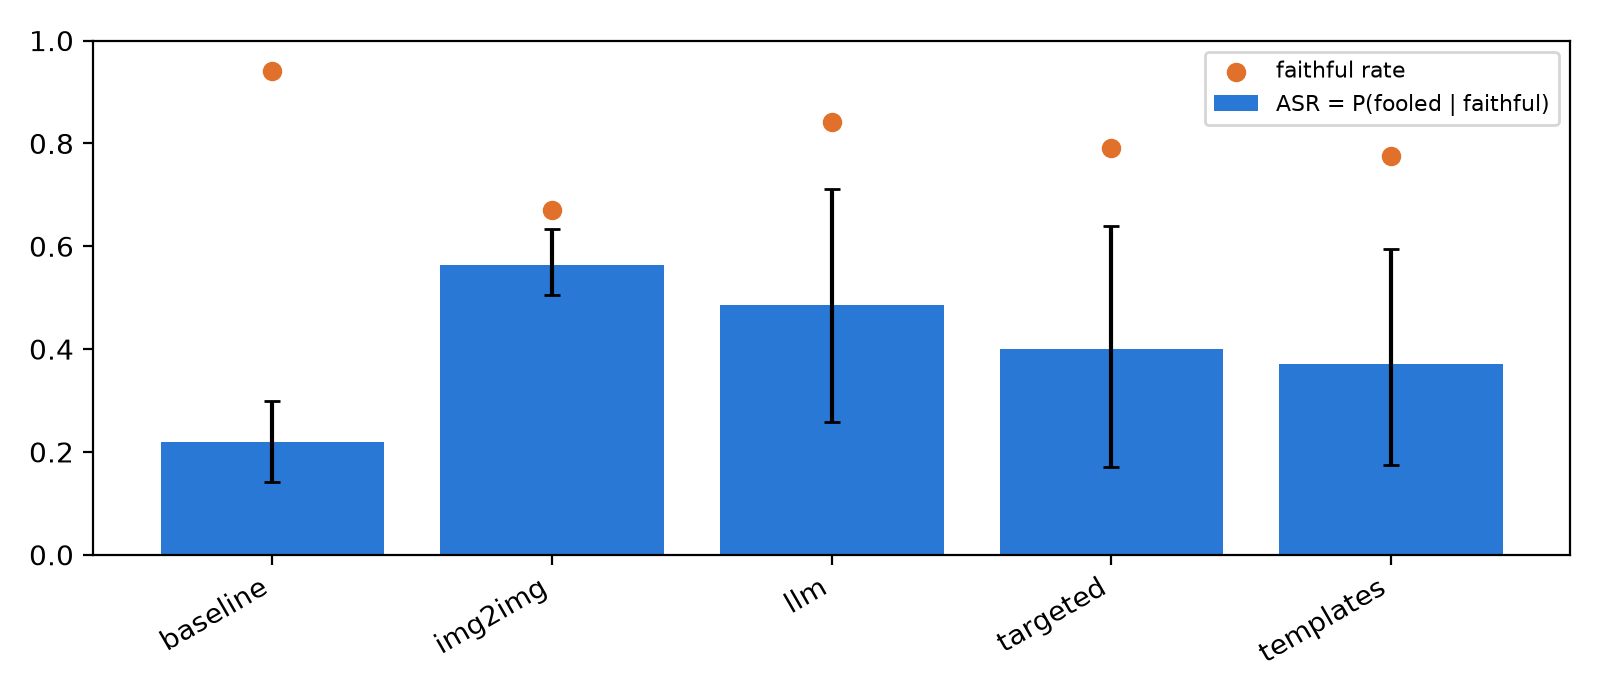
\includegraphics[width=\columnwidth]{../results/figures/asr_by_method.png}
\caption{ASR (bars, 95\% CI) and faithful rate (dots) per method.}\label{fig:asr}
\end{figure}
\begin{figure}[t]\centering
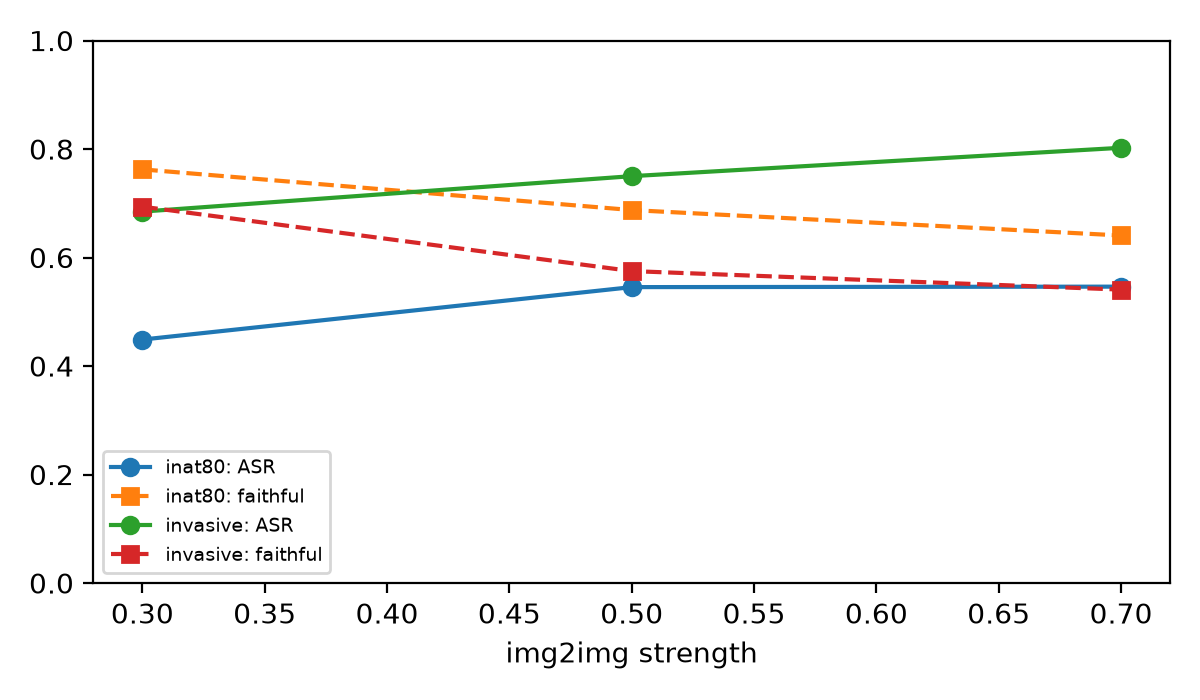
\includegraphics[width=\columnwidth]{../results/figures/img2img_strength.png}
\caption{Editing real photos: ASR and fidelity against the img2img strength.}\label{fig:i2i}
\end{figure}
\begin{figure}[t]\centering
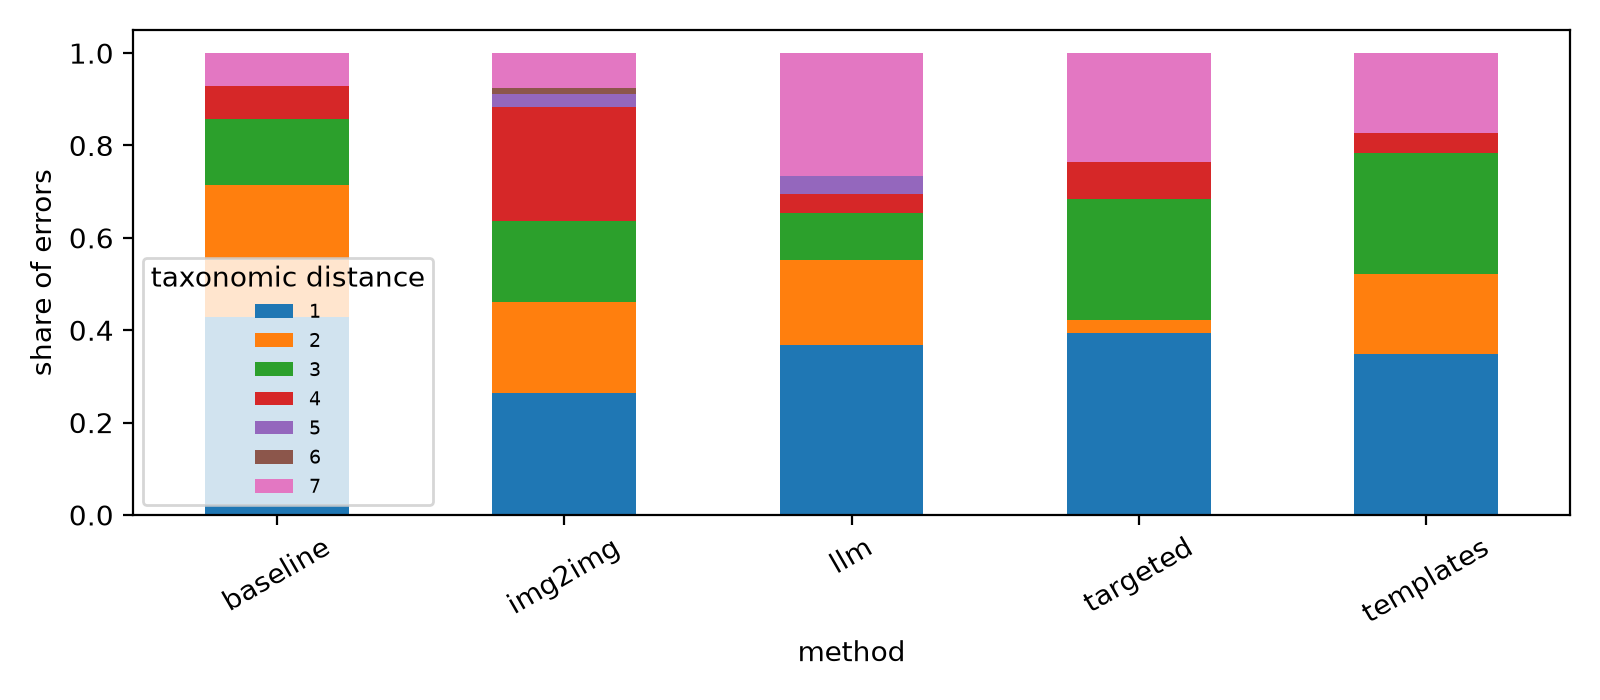
\includegraphics[width=\columnwidth]{../results/figures/taxo_distance.png}
\caption{Taxonomic distance of the errors (1 = same genus, 7 = another kingdom).}\label{fig:taxo}
\end{figure}

\subsection{Post-training}
\todo{DDPO training curves (reward, train ASR, approx. KL) from checkpoints/ddpo/train_log.csv; RAFT vs DDPO vs
best-of-N on split B; LPIPS diversity. The ablation without fidelity: reward hacking examples (figure) and its
faithful rate.}

\subsection{Transfer}
\begin{figure}[t]\centering
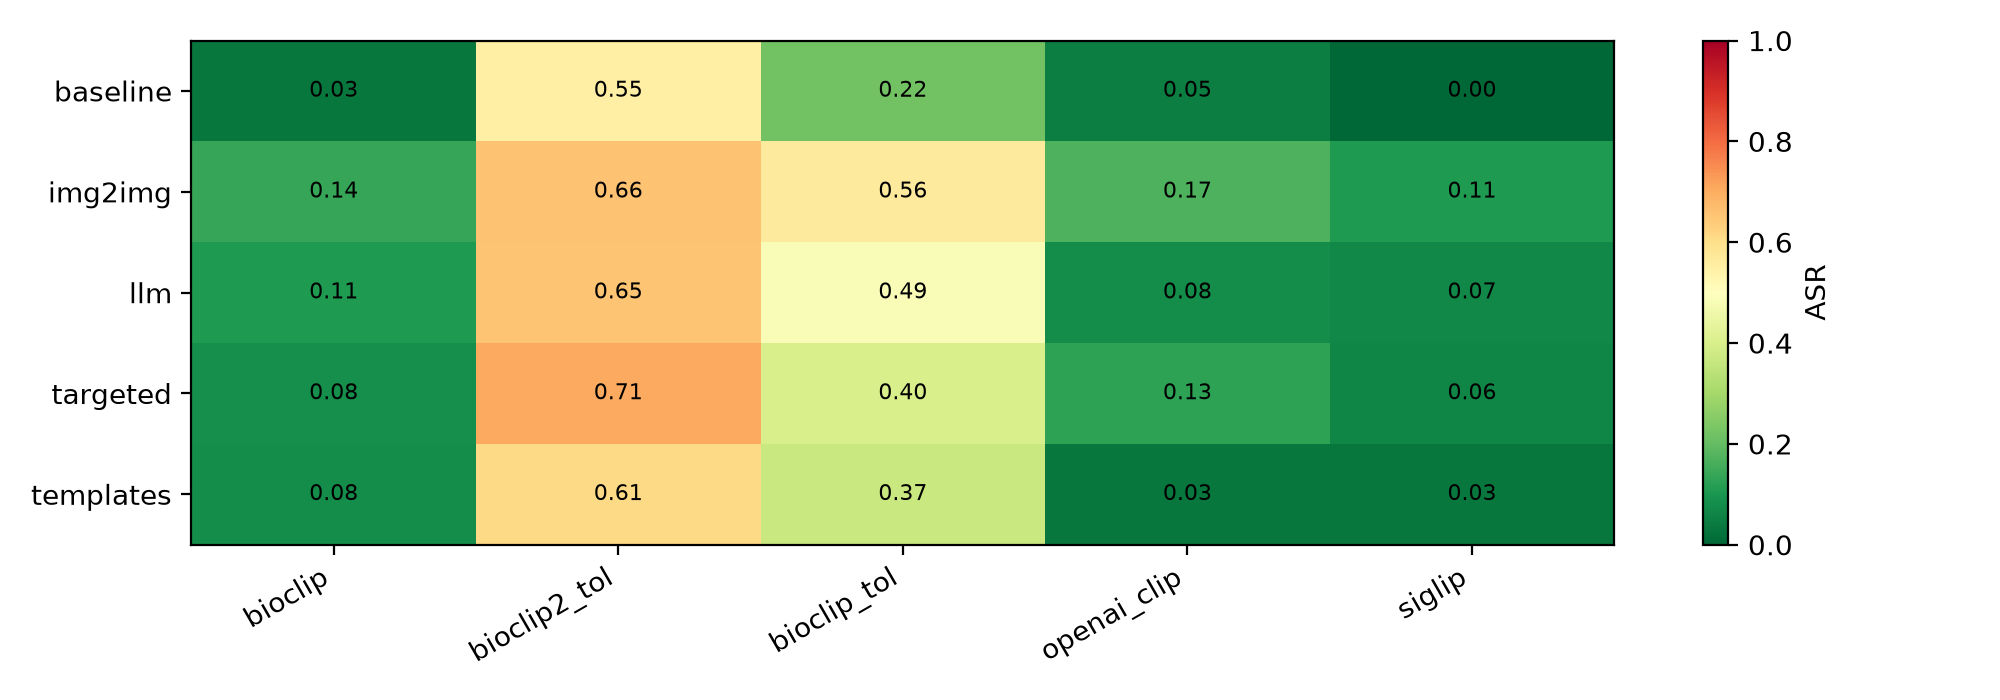
\includegraphics[width=\columnwidth]{../results/figures/transfer_heatmap.png}
\caption{ASR of the same images against other classifiers.}\label{fig:transfer}
\end{figure}
\todo{Do attacks transfer to BioCLIP-2 (the reward oracle, so a biased number), to generic CLIP and SigLIP?}

\subsection{Speed and early rejection}
\begin{table}[t]\centering\small
\caption{Sampling modes: cost and quality.}\label{tab:speed}
\resizebox{\columnwidth}{!}{\input{../results/tables/speed.tex}}
\end{table}
\todo{Table~\ref{tab:speed}: speed-up and quality loss per mode; faithful attacks per GPU-hour. Early rejection:
Spearman correlation between preview and final reward (figures/early_correlation.png), ASR of bon vs bon\_early at
their respective cost. VAE vs TAESD: PSNR and top-1 agreement (outputs/vae/vae\_fidelity.csv).}

\subsection{Why BioCLIP fails}
\todo{t-SNE (figures/tsne\_*.png), layer-wise drift of real vs attacked photos (figures/layer\_drift.png), saliency
examples (figures/saliency\_*.png), confident errors and entropy.}

\section{Discussion and limitations}
\textbf{Oracle bias.} Fidelity is judged by a VLM and by a small human study; both can miss subtle diagnostic
features (wing venation, gill attachment). Our numbers are therefore an upper bound on true fidelity for difficult
groups. \textbf{Generator capacity.} Stable Diffusion 1.5 cannot draw many species; the attackable set and the
img2img attacks address this, but rare species remain under-represented. \textbf{Transfer to BioCLIP-2} is biased
because it is our reward oracle. \textbf{Ethics.} Generated images must not reach citizen-science platforms; we
release the attacks as a benchmark to make BioCLIP more robust, not as a tool to pollute biodiversity data.

\section{Conclusion and future work}
\todo{Two sentences of conclusion.} A natural next step is defence: fine-tuning BioCLIP on the faithful attacks
found here, then measuring robustness and clean accuracy, and attacking newer flow-matching generators.


\bibliography{references}
\bibliographystyle{icml2025}
\end{document}
